%
%  jsag
%
%  Created by franzi on 2013-03-24.
%  Copyright (c) 2013 __MyCompanyName__. All rights reserved.
%
\documentclass[]{article}

% Use utf-8 encoding for foreign characters
\usepackage[utf8]{inputenc}

% Setup for fullpage use
\usepackage{fullpage}

% Uncomment some of the following if you use the features
%
% Running Headers and footers
%\usepackage{fancyhdr}

% Multipart figures
%\usepackage{subfigure}

% More symbols
%\usepackage{amsmath}
%\usepackage{amssymb}
%\usepackage{latexsym}

% Surround parts of graphics with box
\usepackage{boxedminipage}

% Package for including code in the document
\usepackage{listings}

% If you want to generate a toc for each chapter (use with book)
\usepackage{minitoc}

% This is now the recommended way for checking for PDFLaTeX:
\usepackage{ifpdf}

%\newif\ifpdf
%\ifx\pdfoutput\undefined
%\pdffalse % we are not running PDFLaTeX
%\else
%\pdfoutput=1 % we are running PDFLaTeX
%\pdftrue
%\fi

\ifpdf
\usepackage[pdftex]{graphicx}
\else
\usepackage{graphicx}
\fi
\title{Macaulay2 Web Version}
\author{Lars Kastner\\ Freie Universit\"at Berlin \and 
Franziska Hinkelmann\\Mathematical Biosciences Institute\\ Ohio State University \and 
Michael Stillman\\Cornell University  }

\date{}

\begin{document}

\ifpdf
\DeclareGraphicsExtensions{.pdf, .jpg, .tif}
\else
\DeclareGraphicsExtensions{.eps, .jpg}
\fi

\maketitle


\begin{abstract}
\end{abstract}

\section{Introduction}

\begin{figure}[htb]
    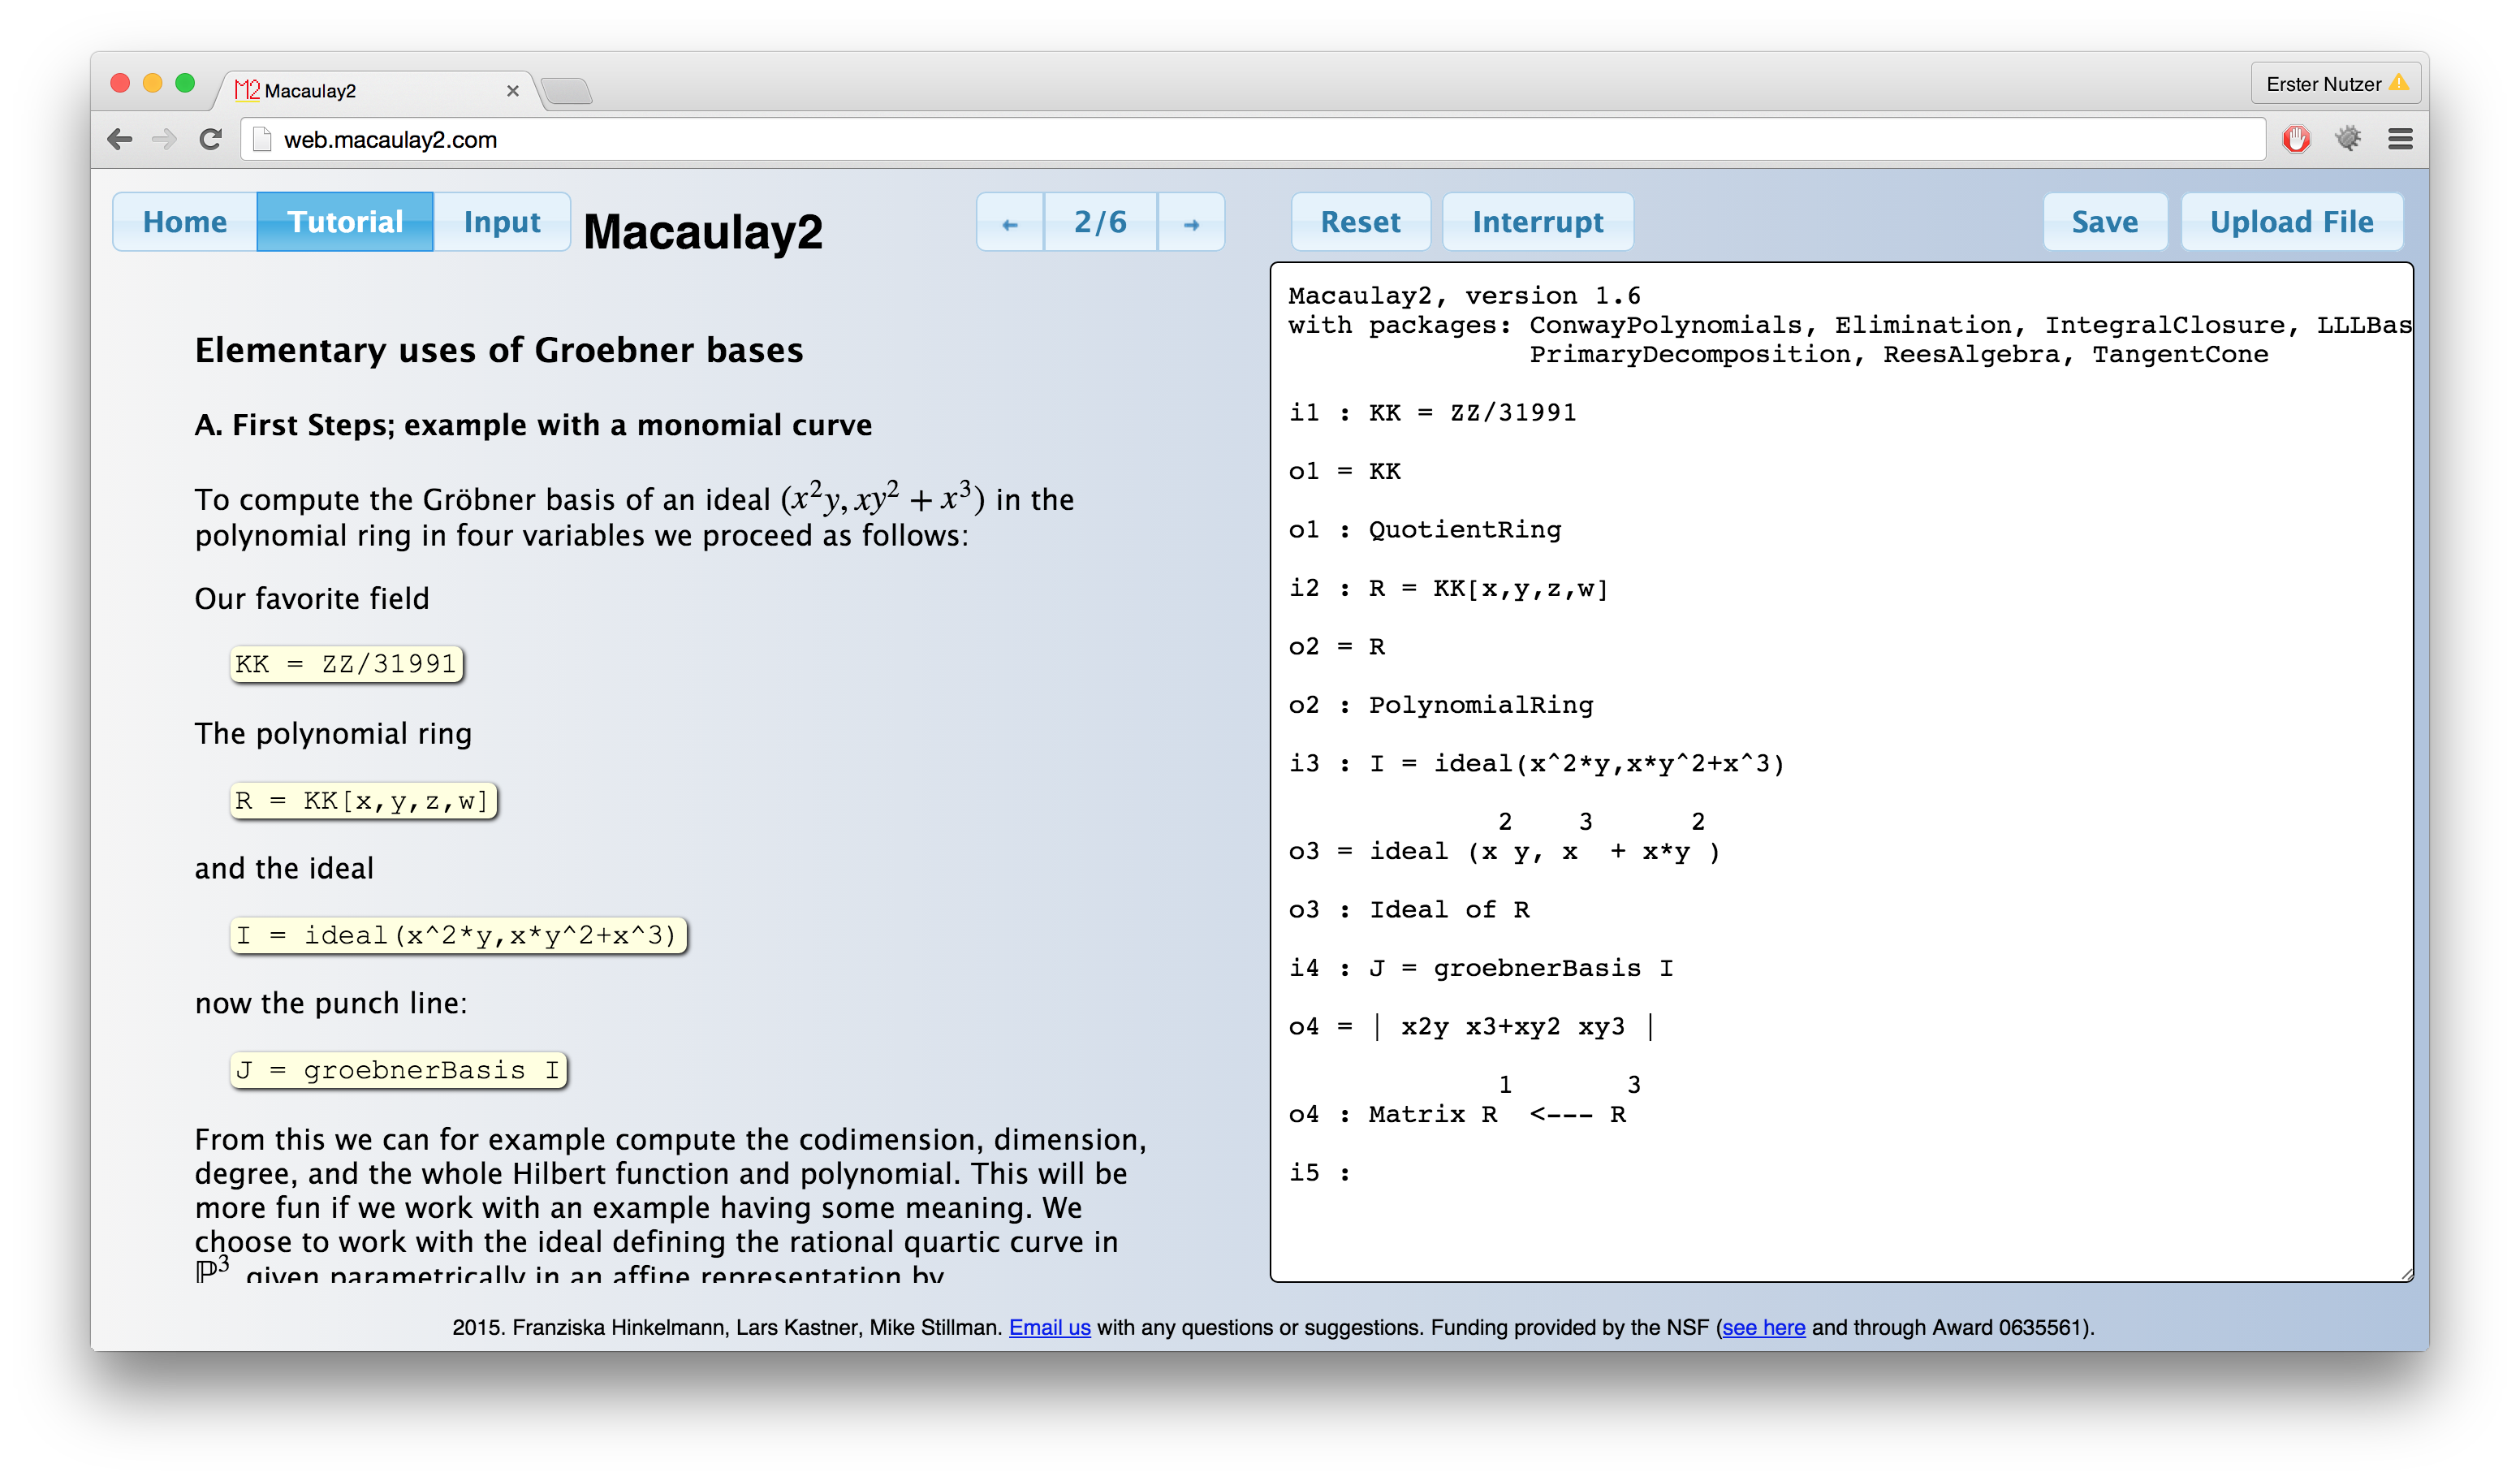
\includegraphics[width=.95\textwidth]{homeWebsite.jpg}
    \caption{Welcome screen of web version of Macaulay2. The left hand side shows a tutorial giving an introduction to Gr\"obner bases. Text in yellow can be clicked and is then executed by Macaulay2 on the server. The complete output of the calculations is show on the right hand side. {\it Home, Tutorial, Input} let the user change the left hand view, {\it Reset, Interrupt} allow to reset and interrupt the Macaulay2 session on the server, {\it Save}  provides both the input and the output of the current session to the user as a text file, and with {\it Upload} one can upload files that can then be accessed by Macaulay2.}
    \label{fig:home}
\end{figure}

The online version of Macaulay2 has the same functionality as regular Macaulay2, albeit the user has access to less resources than on his own machine. The user can upload files and load packages, generate files such as images, and has access to shell commands. 



Motivation (simple for students, simple interface, no time for installation in class, also usable for advanced users (no limitations), other sites (Sage) had heavier interface)
\section{How to use the website}




On the left hand side, the user can navigate between {\it Home}, {\it Tutorial}, and {\it Input}. {\it Home} shows the table of contents of tutorials. {\it Tutorial} shows the currently selected tutorial. Tutorials are interactive and contain executable pieces of Macaulay2 code that are run by clicking on them. {\it Input} shows a terminal window in which the user can type commands and execute them.  

The right hand half shows the output of a Macaulay2 terminal. All code executed either by clicking on interactive parts in a tutorial or by entering code in the {\it Input} window, appears on the right hand side together with the output from Macaulay2 to those results. 

The {\it Reset} button resets a Macaulay2 session, i.e., stopping a running calculation, deleting all variables, unloading all packages, and loading the standard packages. 

The {\it Interrupt} button stops a running calculation, without resetting the Macaulay2 session. 

\subsection{Features}
The user can run all Macaulay2 commands that are available in the running version. To obtain the current version running on the server, type {\tt version}. Loading packages is possible, too, with commands such as {\tt loadPackage}. If packages are not available, they can be uploaded to the users session, by clicking the {\it Upload file} button. Similarly, any other file, such as text files, that one might want to manipulate or read data from with Macaulay2 can be uploaded to the user's session. 

\begin{figure}[htb]
    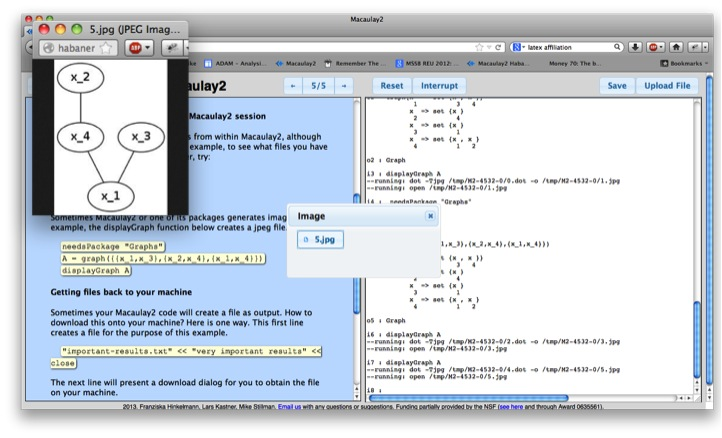
\includegraphics[width=.95\textwidth]{withGraph.jpg}
    \caption{Screenshot of webversion of Macaulay2 after the user generated an image. Some Macaulay2 packages can generate graphs. By invoking the command {\tt displayGraph}, the image is generated on the server and displayed to the user.}
    \label{fig:graph}
\end{figure}

Results from a session can be retrieved by using the {\it Save} button. If the user needs to retrieve files, that are stored in his session, those can be retrieved by executing {\tt open} in the user's session. If Macaulay2 generates graphs, those are shown to the user, see Figure \ref{fig:graph}.

Session are usually being kept alive for several days, which allows users to continue their work next time they access server. 


\section{Tutorials}
writing new tutorials,
\section{Internal structure, schroots}

One of the first questions that occurred to us in this context was whether to offer a sandboxed version of M2 or M2 with full functionality.
We settled for the second alternative, since it seemed easier to realize and more likely to attract new users.
This lead to several new questions:
\begin{enumerate}
\item A fully functional M2 also gives the user system access. How does that impact security and how to deal with it?
\item How do we distinguish the users on the system?
\item How can we limit resources to prevent one user from breaking the system? e.g. via fork bombs.
\item How do we clean up after a user has left?
\item blablabla?
\end{enumerate}

The answer to the second question was to create and delete users on the fly. Since this implies that the server must be run as root, we decided to run it inside a virtual machine in order not to compromise the security of the host system.


Since any system command can be run from inside M2 which is why we decided to run M2 inside a `secure chroot' (schroot). To provide full funtionality we mount a full system inside the schroot. The mounting happens read only, a few folders are provided with a writable layer, if M2 needs write access to them. In the definition of a user specific schroot there is not root user, so it should not be possible to become root or execute any command via sudo.

When a user connects to the server the following things happen:
\begin{enumerate}
\item A user account on the system is created.
\item A schroot configuration file is created with the above user as only user.
\item Control groups for memory and CPU are created.
\item The schroot is started.
\end{enumerate}

Control groups (cgroups) allow you to restrict the number of CPU shares and the memory for a process and all its children. When M2 is executed inside a schroot it is called via {\tt cgexec} with the cgroups specifically created for this user. Using this technique it is possible to limit the total consumption of CPU and memory by each user. Additionally we ensure that the administrator of the virtual machine always is able to execute any command required for maintenance, i.e. if the node server is down or has been compromised.

Now any Macaulay2 command can be run in this schroot inside the corresponding cgroups.

Lars!
link to tutorial from Lars for setting up your own server, link to github



\bibliographystyle{plain}
\bibliography{}
\end{document}
